
\documentclass{article}  

%
\usepackage{graphicx}
%%%%%%%%%%%%%%%%%%%%%%%%%%%%%%%%%%%%%%%%
\usepackage{txfonts}
%%%%%%%%%%%%%%%%%%%%%%%%%%%%%%%%%%%%%%%%
\usepackage{mathrsfs}
\usepackage{mathtools}
\usepackage{svg}
\usepackage{hyperref}





\newenvironment{boxed2}
    {\begin{center}
    \begin{tabular}{|p{0.45\textwidth}|}
    \hline\\
    }
    { 
    \\\\\hline
    \end{tabular} 
    \end{center}
    }

%%Define floor and ceiling function notation below
\DeclarePairedDelimiter\ceil{\lceil}{\rceil}
\DeclarePairedDelimiter\floor{\lfloor}{\rfloor}

% To add links in your PDF file, use the package "hyperref"
% with options according to your LaTeX or PDFLaTeX drivers.
%
\begin{document} 


   \title{Crystal Hypergraph Convolutional Networks}
   
   \subtitle{}

   \author{Alexander Heilman
          }

   \institute{Northeastern University\\
             Boston, Massachusetts}

   \date{\today}

 
  \abstract{
  Hypergraphs are a natural extension of the common graph structure that allow
  for the association between arbitrary numbers of nodes in a set 
  of hyperedges. By applying these structures as a representation of crystalline
  unit cells, we can apply a hypergraph neural network to learn representations
  for crystalline sites, bonded pairs, and higher order structures of crystals 
  (i.e. motifs) simultaneously.
  }

   \keywords{Hypergraph neural network, crystal hypergraph, crystal hypergraph convolutional neural network}

   \maketitle
%
%-------------------------------------------------------------------
\section*{Terminology}
A \textit{hypergraph} is a set of a set of nodes, or vertices, and a set
of hyperedges, which are subsets of the set of nodes of arbitrary size (as
opposed to graph edges, which only connect two).
We term these hyperedges \textit{hedges} for
brevity.

The \textit{relatives graph} is a novel construction, derived from an underlying hypergraph and a binary relation between distinct hyperedges. In this relatives graph, nodes represent hyperedges and edges represent that those hyperedges are related in their underlying hypergraph.



\section*{Introduction}
By encoding crystalline structures as hypergraphs, and applying representational
learning to those hyperedges in a graph convolutional network, we may effectively learn representations for all orders of structures in a crystal simultaneously. 


As an example, in contrast to the common node representation scheme; in a hypergraph structure we may simply adjoin the singleton sets to the hyperedge list to effectively learn the same representations.

%%%%%%Layout%%%%%%%%%%%%%%
%Explain concept high level
%%%%Motivate from motifs +
%%%%Atoms as singletons
%%%%Natural higher-order representations 

%Define construction of crystal hypergraphs
%%%%Simplest approach: tiered Voronoi + 
%%%%   conditions (solid angle, scaled min distance cutoff)
%%%%Initialization of node features (singleton set feature vectors)

%Overview HGCONV network actions and define model structure
%%%%Explain pyg hyperconv function
%%%%Explain model architectures used

%Data and results
%%%%Formation energy per atom
%%%%Energy above hull
%%%%Band gap
%%%%Is metal?

%HG Attention 
%%%%See which order structure was most informative

%Wrap up and out look
%%%%%%%%%%%%%%%%%%%%%%%%%%%%%%

\section{Motivation \& Overview}
The modelling of crystalline structures as graphs in Graph Neural Networks (GNNs) has shown widespread success in the prediction of material properties. The most notable examples include the widely acclaimed Crystal Graph Convolutional Network (CGCNN \cite{xie2018crystal}), Material Graph network (MEGNet \cite{chen2019graph}), and atomistic line graphs (LINE \cite{choudhary2021atomistic}).
. 
In such models, crystalline systems are converted to graphs by treating atoms as nodes and bonds or connections as edges (usually determined solely on distance). The graphs derived in this manner then have relevent atomic properties associated with their nodes in the form of feature vectors, and the edges are generally endowed with feature vectors encoding their properties (essentially just distance).

One limitation of such structures though, is the restriction to strictly pair-wise descriptors. This only allows one to associate, at most, features to the atomic sites themselves and the bonds between them. This obviously lacks the detail of the larger geometric properties of the structure. This pair-wise limitation may even be particularly problematic in certain crystalline structures known to have higher order structures, and hence correlations, such as the well-known motifs present in complex oxides and other minerals (like those discussed in Pauling's rules). 

More recent progress has been made in networks that take advantage of these higher order structures, such as motif-level \cite{banjade2021structure} and triplet-level \cite{choudhary2021atomistic} adjacent graphs
which can incorporate more geometrical information in the initial features.
Based on these advancements, we propose a new framework that models crystals as hypergraphs, which naturally allow for the encoding of higher order correlations in representation learning. These crystal hypergraphs are constructed iteratively such that each hyperedge is associated with a certain order of structure (one node, two nodes, three, etc.), and so each order naturally represents a different level of structure within the crystal (respectively atoms, pairs, and triplets, etc.). We then associate an order-dependent type of feature with each hyperedge.

While regular hypergraph convolution may then be performed on these natural crystal hypergraphs, as in \cite{jo2021edge}
, we propose a further method of construction that allows one to perform the more common techniques of Message Passing Neural Networks (MPNN) on a "relatives graph" defined from the crystal hypergraph.

This relatives graph is inherited from the crystal hypergraph via some relation function between hyper edges, where the most intuitive is inclusion. That is, two hyperedges are deemed to be related, and hence have an edge between their respective nodes in the relatives graph, if one is contained within the other. The relatives graph is naturally heterogeneous with different node types for the different orders of structures

This relatives graph is then passed to a MPNN which may be trained to learn arbitrary material properties. While the chosen MPNN functions may be chosen freely from those previously used, in this new structure we have a novel pooling method: for crystal-level predictive tasks, we may further add a 'crystal node' that is connected to every hedge node in the relatives graph. This crystal node may then be taken as the learned representation vector for the entire crystal, and from which most tasks the relevant information may be drawn from using the usual MLPs. In this way the learned crystal vector (via the MPNN) may be naturally extracted from all relevant substructures of the crystal. This stands in opposition to the more agnostic pooling functions usually employed, such as averaging and summing.

Below, we give a brief overview of common crystal graph construction techniques and then propose a crystal hypergraph construction technique. We then show how to construct an equivalent heterogeneous graph from the hypergraph, and use that as input into a heterogeneous graph network.

Results are then presented for different combinations of orders of structures in the prediction of common material properties.


\begin{boxed2}
    \textbf{Note: Equivalence of Hypergraph Convolution on Hyperedges and Message Passing on Relatives Graph} 

    \medskip
    
    Once the relations between hyperedges are determined, all that needs to be done is the relevant representations need to communicate via some defined structure. Of course, once the related hyperedges for every hyperedge are determined 
\end{boxed2}

%%%%%%%%%%%%%%%%%%%%%%%%%%%%%
%%Motivation for edge representations%
%%%%%%%%%%%%%%%%%%%%%%%%%%%%%
%Requires defining new convolutional structure%

\section{Crystal Graphs}
In the usual techniques of material property prediction that utilize graph convolutional networks, we first need to define what the graphs are.

To do this, we essentially just need to define what out nodes are (atoms); what are edges are (by some physical criteria); and what features we should associate with both. 

The nodes are simply the atoms of the structure. 
Most constructions then take the simple approach of creating an edge between two atoms if their inter-atomic distance is below some threshold (6-10 Ang), and  truncating the number of edges for each node at some maximum number of neighbors (usually 12). 

The associated features for the atoms or nodes then are usually based only on the atomic number of the site. A common set of atomic number dependent feature vectors is that proposed in CGCNN. 
Edges then have their distance encoded in their respective feature vectors, usually in a Gaussian expansion (to increase the dimensionality and hence weight of this attribute).
\begin{center}

\end{center}
Two notable examples of additions: MEGNet further associated a 'state-level' feature with the entire graph, which encoded thermodynamic properties; and LINEGraph generated a second graph for every crystal graph, termed the 'line graph' which could encode bond angles as an additional feature. We will show that these two implementations are special cases of the hypergraph framework we propose.

\section{Implementation}
Having now given a brief overview of the constructions proposed, we proceed to the specific implementation below

\subsection{Crystal Hypergraph Construction}
In Graph Networks, the more often used approach is to learn representations solely of nodes as is the approach taken in most previous works \cite{choudhary2021atomistic, xie2018crystal, banjade2021structure, chen2019graph}. 

But, a more robust and informative representation leveraging the multi-order structures encoded in hypergraphs may be achieved in a novel edge-representation learning structure. So in the hypergraph construction below, we rather associate features with hyperedges. Furthermore, we allow for different dimensional features for each order of representations. 

As mentioned before, we choose a iterative construction process, allowing for a modular approach that can fully leverage the freedom in representation between different order hyperedges.

For the specific implementation tested giving the results presented later, we choose a three layer hypergraph construction process for crystalline structures. The first order of structures being singleton edges representing atoms; second being pairs representing bonded atoms; and third, hedges containing all nearest neighbors of each site, with these representing structures analogous to motifs.

To further take advantage of these structures we also include a "master hyperedge" which contains all nodes. This master hedge will be used to represent the entire structure for graph-level tasks, usurping the usual pooling functions (which usually take the mean, max, or minimum node-level representation as the learned graph-level representation).

\subsubsection{Node/Atom Hyperedges}
To treat atoms in the same way as edges and higher order structures, we may represent atom's as hyperedges that contain exactly one atom. These are hyperedges that are singleton sets. We then associate the atom's representation through learning with these singleton edges. As such, the initial features of such edges may be the usual atom features used in crystal graph neural networks, such as the encoding used in the CGCNN framework.

\hspace{-.25cm}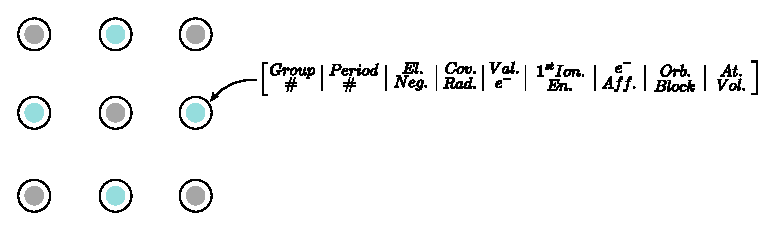
\includegraphics[scale=0.65]{singleton.pdf}

This is perhaps the simplest step of construction since essentially no parameters must be associated with the process, in that each node simply gets it's own singleton hedge.


\subsubsection{Edge/Pair Hyperedges}
We then construct the usual pair-wise edges.  Inspired by previous work, we may simply take their initial features to be a Gaussian expansion of the inter-atomic distance (8 dimensions).

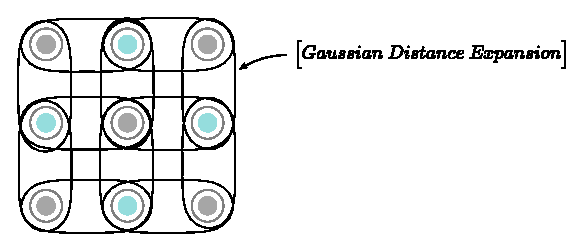
\includegraphics[scale=0.74]{pair.pdf}

These edges may be constructed the usual way, by using a maximum inter-atomic distance cut off and only allowing for a certain number of total bonded atoms (12) for each atom.


\subsubsection{Nearest Neighbors/Motif Hyperedges}
Higher order edges are perhaps the most interesting component of the novel model, and allow for the correlation of representations for larger substructures within the unit cell. For the model at hand, we consider hyperedges contains all sets of nearest neighbors (as well as their respective centers). These nearest neighbors are selected according to some scalar value multiplied by the minimum inter-atomic radii of the center (we neglect the additional solid angle criteria for simplicity).

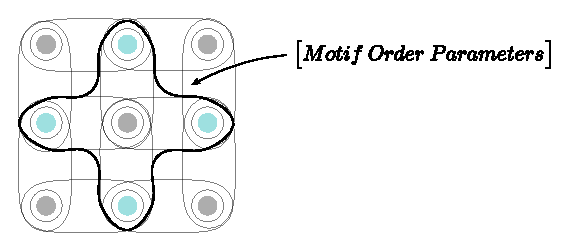
\includegraphics[scale=0.74]{motif.pdf}

These bonafide hyperedges require a more subtle application of feature engineering, though some previous work is used as inspiration, such as \cite{zimmermann2020local}. For now, we use a list of local structure order parameters as initial features, which we calculate with the package implemented in pymatgen.


Note that previous work, such as in \cite{choudhary2021atomistic}
, this higher order structure was essentially used to represent triplets of atoms, and where representations were expansions of bond angles. This additional geometrical information resulted in cutting-edge performance in most predictive tasks of material properties.

  
\subsubsection{Master/Crystal Hyperedge}
We then associate a hyperedge containing and representing the entire crystalline structure to be used for graph-level prediction tasks after training. 

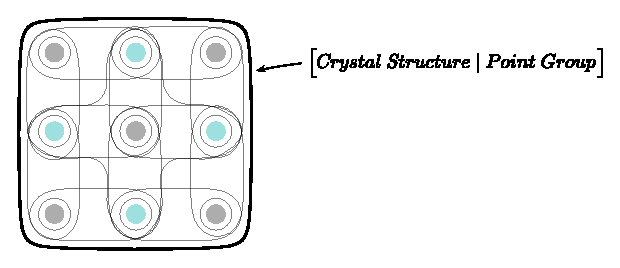
\includegraphics[scale=0.74]{master.pdf}

For now, we start with a randomly initialized representation, though information such as crystalline point group, symmetries, and underlying crystalline structure may be useful to include in the initial feature.

\subsection{Relatives Graph Construction}
The trick now is to relate this hypergraph structure to a graph (or, more naturally, a heterogeneous graph), so that the usual techniques of MPNNs may be applied. Indeed, this is equivalent to convolution over the hypergraph (given an appropriately define binary relation between hyperedges), since message passing essentially allows for arbitrary forms of information to be communicated between each node and all it's related nodes. Furthermore, this conversion allows us to take advantage of most previous work's convolutional layers.


\begin{figure*}[htbp]
  \centering
  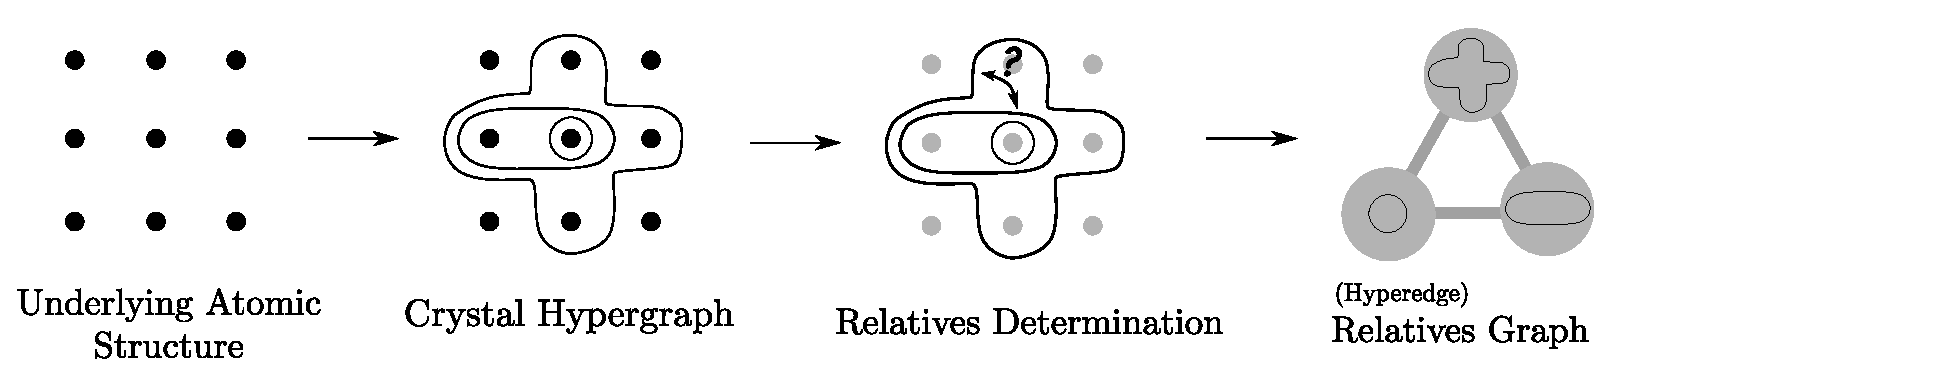
\includegraphics[scale=.48]{relgraph_workflow_horiz.pdf}
  \caption{Schematic overview of workflow}
\end{figure*}

The relatives graph construction may essentially be taken as an extra preliminary step to the usual MPNN workflow as defined in%Gilmore
. This first step requires we define some binary relation between hyperedges, so that we may determine whether two hyperedges are related. We may apply this relation to all pairs of hyperedges then to return a relatives graph, where nodes represent hyperedges and edges represent that two connected nodes are two hyperedges that are related to each other and hence should communicate through message passing.

\subsection{Network Architecture}

The relatives graph essentially just defines those representations to aggregate for each hyperedge's message which is passed in each layer.
Thus, once the relatives graph has been defined, we may simply pass this new structure to the archetypal message passing layers, albeit with no edge features. 
Thus, our total architecture allows us to apply those convolutional structures usually applied in such tasks (such as CGConv w/ no edge features, TransformerConv, SAGEConv).

 Before the graph-convolutional layers, however, we must homogenize the initial features, since the different order structures naturally have different dimensional representations. This is done by a simple, trainable projection layer associated with each class of structure/order of hyperedge. This projection layer is just a learned matrix multiplied by the corresponding input (foregoing the usual non-linear activation function that follows in each NN layer).

We now pass these relatives graphs to the chosen MPNN. In the model tested, after projection to a homogeneous hidden hedge representation of 64 dimensions, each layer is passed through 3 SAGEConv graph-convolutional layers, the representations of all the hedges are then mean pooled, the result over which is passed to a MLP layer of depth 128 with a softplus activation function. This outputs a one-dimensional scalar predicting the corresponding material property.


\begin{boxed2}
    "
    One reason is that the standard GNNs cannot distinguish certain types of graphs relevant for chemistry is they cannot distinguish molecules like decaline and bicylopentyl, which indeed have different properties. Look at the Fig. 24.1 below and think about the degree and neighbors of the atoms near the mixing of the rings – you’ll see if you try to use message passing the two molecules are identical. This is known as the Wesifeiler-Lehman Test [WL68]." from \url{https://dmol.pub/dl/molnets.html}


    This approach, proposed here may pass the Wesifeiler-Lehman Test?
\end{boxed2}


%%Gaussian Expand LSOP features?
%%Associate graph-level edge
%%Use learned graph-level edge rep as learned crystal rep
%%Use line graph and Megnet as examples of general structure



\nocite*
\bibliographystyle{plain} % We choose the "plain" reference style
\bibliography{chgcnn} % Entries are in the refs.bib file

\end{document}